\documentclass{article}

\usepackage{graphicx}
\usepackage{amsmath}
\usepackage{fancyhdr}
\usepackage{listings}
\usepackage[sorting=none]{biblatex}
\usepackage[margin=1in]{geometry}
\usepackage[font={small,it}]{caption}
\usepackage{placeins}
\usepackage{xepersian}

%\DeclareMathOperator*{\btie}{\bowtie}
\addbibresource{bibliography.bib}
\settextfont[Scale=1.2]{B-NAZANIN.TTF}
\setlatintextfont[Scale=1]{Times New Roman}
\renewcommand{\baselinestretch}{1.5}
\pagestyle{fancy}
\fancyhf{}
\rhead{تکلیف دوم درس پایگاه داده‌ها 1}
\lhead{\thepage}
\rfoot{علیرضا ابره فروش}
\lfoot{9816603}
\renewcommand{\headrulewidth}{1pt}
\renewcommand{\footrulewidth}{1pt}

\begin{document}
\begin{titlepage}
\begin{center}

\includegraphics[width=0.4\textwidth]{figures/IUT Logo.png}\\
        
\LARGE
\textbf{دانشگاه صنعتی اصفهان}\\
\textbf{دانشکده مهندسی برق و کامپیوتر}\\
        
\vfill
        
\huge
\textbf{عنوان: تکلیف چهارم درس ریزپردازنده}\\
        
\vfill
        
\LARGE
\textbf{نام و نام خانوادگی: علیرضا ابره فروش}\\
\textbf{شماره دانشجویی: 9816603}\\
\textbf{نیم\,سال تحصیلی: پاییز 1400}\\
\textbf{مدرّس: دکتر عارف کریمی افشار}\\
\end{center}
\end{titlepage}


%\tableofcontents
\newpage

\section{}
\begin{table}[ht]
    \centering
    \begin{tabular}{|c|c|c|}
    \hline
    \textbf{داده} & \textbf{نوع متغیر(\lr{int}، \lr{varchar}، \lr{char}، $\ldots$)}\\
    \hline
    سه حرف مخفف شده ماه‌های میلادی & \lr{char}\\
    \hline
    قیمت دلاری محصولات که همگی دو رقم اعشار دارند &\lr{numeric}\\
    \hline
    نام و نام خانوادگی کاربر & \lr{varchar}\\
    \hline
    کد ملی کاربر & \lr{char}\\
    \hline
    ذخیره قیمت لحظه‌ای ارز‌های دیجیتال دلار & \lr{real, double precision}\\
    \hline
    تعداد بازدید یک ویدئو & \lr{int}\\
    \hline
    \end{tabular}
    \caption{جدول شماره 1}
    \label{tab:tab1}
\end{table}


\section{}
\begin{figure}[ht]
    \centering
    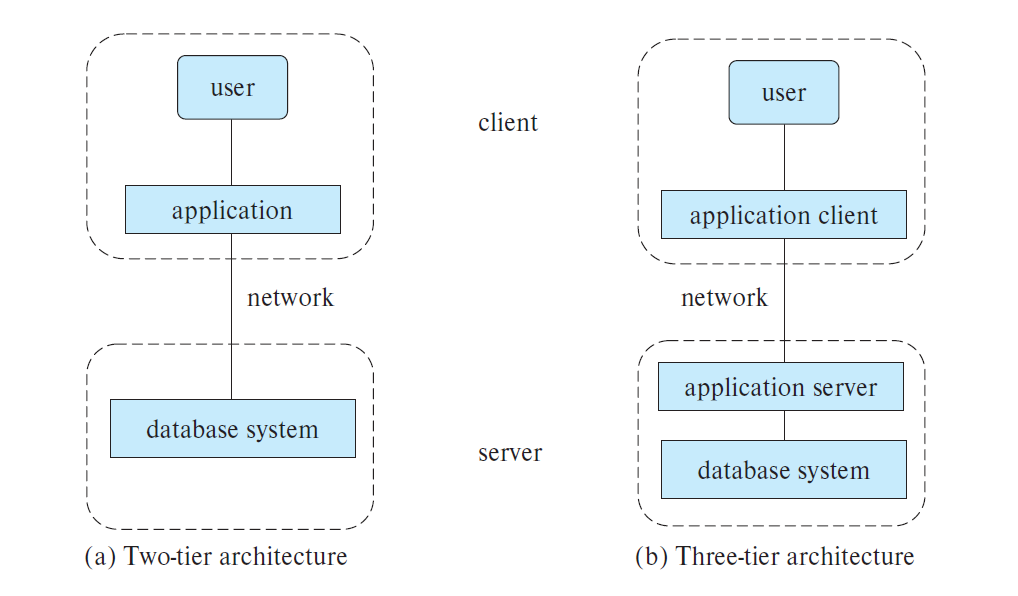
\includegraphics[width=0.8\textwidth]{figures/2.png}
    \caption{}
    \label{fig:fig1}
\end{figure}
\FloatBarrier
\begin{table}[ht]
    \centering
    \begin{tabular}{|c|c|c|}
    \hline
    \textbf{ویژگی‌ها} & \textbf{معماری دولایه} & \textbf{معماری سه‌لایه}\\
    \hline
    سرعت & کمتر(کندتر) & بیشتر(سریعتر)\\
    \hline
    امنیت & کمتر(کلاینت می‌تواند مستقیما با پایگاه داده تعامل داشته باشد) & بیشتر(کلاینت مجاز به تعامل مستقیم با پایگاه داده نمی‌باشد)\\
    \hline
    افزونگی & کمتر & بیشتر(چون تعداد لایه‌ها بیشتر است در نتیجه \lr{indirection}ها بیشتر است)\\
    \hline
    مقیاس‌پذیری & کمتر & بیشتر(به دلیل ماژولارتی بالا امکان\lr{maintainance} آن بیشتر است)\\
    \hline
    انعطاف‌پذیری & کمتر & بیشتر(امکان افزودن \lr{feature} در آن ساده‌تر است)\\
    \hline
    یک‌پارچگی & کمتر & بیشتر(به دلیل لایه‌ای بودن یک‌پارچگی بیشتر حفظ می‌شود)\\
    \hline
    \end{tabular}
    \caption{جدول شماره 1}
    \label{tab:tab1}
\end{table}

\section{}
\subsection{}
	\centering
\lr{WHERE 1 <= (SELECT count(name) FROM student)}

\subsection{}
\lr{attribute}های
مشخص شده در قسمت قبل با کاراکتر
\lr{\#}
و
\lr{@}
به ترتیب بیانگر کلید اصلی بودن و کلید خارجی بودن در آن جدول اند.

\section{}
\subsection{}
مقدار خاص
\lr{null}
که در هر
\lr{domain}
قرار دارد(به جز مواردی که خود ما محدود کرده باشیم) به این معنی است که ما اطلاعی راجع به این فیلد نداریم. توجه شود که
\lr{null}
با صفر متفاوت است. برای مثال اگر حقوق یک کارمند صفر باشد به این معنی است که جمع دریافتی‌ها و کسری‌های او صفر می‌شود، درحالی که اگر حقوق او
\lr{null}
باشد به این معنی است که اطلاعی از حقوق او در پایگاه داده موجود نیست. همچنین در پایگاه داده‌ی دانشگاه،
\lr{null}
بودن نمره یک دانشجو به معنی موجود نبودن(وارد نشده بودن) آن در پایگاه داده‌ی دانشگاه است.
\subsection{}
می‌توان یک
\lr{relation schema}
به نام
\lr{employment}
با
\lr{attribute}های
\lr{i\_id}
که شناسه استاد،
و
\lr{dept\_name}
که نام دانشکده است،
به شکل زیر تعریف کرد:
\begin{center}
\begin{tabular}{|l|} \hline
    \textbf{\lr{employment}} \\ \hline
    \lr{i\_id} \\ \hline
    \lr{dept\_name} \\ \hline
\end{tabular}
\end{center}
به این شکل می‌توانیم
\lr{dept\_name}
را از
\lr{instructor}
حذف کنیم و رابطه‌ی اشتغال را بین دانشکده و استاد برقرار کنیم(شبیه کاری که برای استاد راهنما انجام شد). از این طریق در پایگاه داده یک استاد می‌تواند در بیش از یک دانشکده مشغول به کار باشد.

\subsection{}
یک راه می‌تواند اضافه کردن یک
\lr{attribute}
تحت عنوان
\lr{second\_advisor}
به
\lr{advisor}
باشد. از آنجایی که می‌دانیم هر دانشجو حداکثر می‌تواند دو استاد راهنما داشته باشد، در صورتی که دانشجو یک استاد راهنما داشت، تنها از
\lr{first\_advisor}
استفاده کنیم و فیلد
\lr{second\_advisor}
برابر
\lr{null}
قرار دهیم.
\subsection{}
اگر یک رکورد از
\lr{student}
حذف شود، آنگاه رکورد مربوط به رکورد حذف شده در
\lr{takes}
نامعتبر خواهد بود. همچنین درصورتی که یک رکورد با
\lr{ID}
ناموجود وارد شود دچار نقض می‌شود.
 

\section{}
\subsection{}
$
\Pi_{Title,\:ReturnDate}
(Borrow \bowtie_{MemberID\:=\:1356\:\wedge\:IsReturned\:=\:false} Book)
$

\subsection{}
$
\Pi_{Name}
(Member
\bowtie_{Member.CategoryID\:=\:``Physics"}
(Book \bowtie_{Book.BookID\:=\:Borrow.BookID\:\wedge\:CategoryID\:=\:``Physics"}\:Borrow))
$
\subsection{}
$
\Pi_{Name,\:Title}
(Member
\bowtie_{Member.CategoryID\:=\:Book.CategoryID}
Book)
\:-\:
\newline
\Pi_{Name,\:Title}
(Borrow
\bowtie_{Borrow.MemberID\:=\:Member.MemberID\:\wedge\:Borrow.BookID\:=\:Book.BookID}
\newline
(Member
\bowtie_{Member.CategoryID\:=\:Book.CategoryID}
Book))
$
\subsection{}
$
\Pi_{Name,\:Title}
(Member
\bowtie_{Member.MemberID\:=\:Borrow.MemberID}
\newline
(Borrow
\bowtie_{CategoryID\:=\:``Drama"\:\wedge\:IsReturned\:=\:false\:\wedge\:Today\:-\:ReturnDate\:>\:10\:Days}
Book))
$
\subsection{}
ابتدا عبارت را به شکل زیر تفکیک می‌کنیم:
\begin{center}
$
D
\leftarrow
Borrow
\bowtie_{Borrow.BookID\:=\:Book.BookID}
Book
$
\end{center}
\begin{center}
$
C
\leftarrow
D
\bowtie_{Borrow.MemberID\:=\:Member.MemberID}
Member
$
\end{center}
\begin{center}
$
B
\leftarrow
\sigma_{Borrow.NumDays\:\times\:Book.Penalty\:\geq\:100000}
(C)
$
\end{center}
\begin{center}
$
A
\leftarrow
\Pi_{Member.Name,\:Book.Title}
(B)
$
\end{center}
\lr{D}
لیست اطلاعات کتاب‌های امانت گرفته‌شده را همراه با اطلاعات امانت آن‌ها برمی‌گرداند.
\newline
\lr{C}
لیست اطلاعات اعضا و اطلاعات کتاب‌های امانت گرفته‌شده آن‌ها را همراه با اطلاعات امانت آن‌ها برمی‌گرداند.
\newline
\lr{B}
سطر‌هایی از
\lr{C}
را برمی‌گرداند که جریمه دیرکرد آن‌ها بزرگتر یا مساوی 100000 تومان باشد. 
\newline
\lr{A}
که همان عبارت نهایی است ستون‌های نام عضو و نام کتاب را از
\lr{B}
برمی‌گرداند.
\newline
پس نتیجه عبارت، نام عضو و نام کتاب‌هایی که امانت گرفته‌اند و جریمه دیرکرد آن‌ها بزرگتر یا مساوی 100000 تومان است می‌باشد.
%%%%%%%%%%%%
\subsection{}
ابتدا عبارت را به شکل زیر تفکیک می‌کنیم:
\begin{center}
$
F
\leftarrow
Book
\bowtie_{Book.AuthorID\:=\:Author.AuthorID}
Author
$
\end{center}
\begin{center}
$
E
\leftarrow
F
\bowtie_{Book.CategoryID\:=\:Category.CategoryID}
Category
$
\end{center}
\begin{center}
$
D
\leftarrow
\sigma_{Category.CategoryName\:=\:``Philosophy"\:\wedge\:Author.Name\:\neq\:``Plato"}
(E)
$
\end{center}
\begin{center}
$
C
\leftarrow
(\sigma_{IsReturned\:=\:false}(Borrow))
\bowtie_{Borrow.BookID\:=\:Book.BookID}
Book
$
\end{center}
\begin{center}
$
B
\leftarrow
\Pi_{Book.Title}(C)
$
\end{center}
\begin{center}
$
A
\leftarrow
\Pi_{Book.Title}(D)
$
\end{center}
\begin{center}
$
A\:-\:B
$
\end{center}
\lr{F}
اطلاعات کتاب‌ها را به همراه اطلاعات نویسنده‌ی آن‌ها برمی‌گرداند.
\newline
\lr{E}
اطلاعات
\lr{F}
را به تفکیک اطلاعات موضوع آن‌ها برمی‌گرداند.
\newline
\lr{D}
سطرهایی از
\lr{E}
با موضوع
\lr{Philosophy}
که نویسنده آن‌ها
\lr{Plato}
نیست را برمی‌گرداند.
\newline
\lr{C}
اطلاعات کتاب‌های امانت داده شده اما بازگردانده نشده اند را برمی‌گرداند.
\newline
\lr{B}
ستون نام کتاب از
\lr{C}
را برمی‌گرداند.
\newline
\lr{A}
ستون نام کتاب از
\lr{D}
را برمی‌گرداند.
\newline
\lr{A\:-\:B}
که همان عبارت نهایی است تفاضل
\lr{B}
از
\lr{A}
را برمی‌گرداند.
\newline
پس نتیجه عبارت، نام کتاب‌هایی با موضوع
\lr{Philosophy}
که نویسنده آن‌ها
\lr{Plato}
نیست و امانت داده شده اما بازگردانده نشده اند را برمی‌گرداند.

\section*{منابع}
\renewcommand{\section}[2]{}%
\begin{thebibliography}{99} % assumes less than 100 references
%چنانچه مرجع فارسی نیز داشته باشید باید دستور فوق را فعال کنید و مراجع فارسی خود را بعد از این دستور وارد کنید


\begin{LTRitems}

\resetlatinfont

\bibitem{b1} https://www.geeksforgeeks.org/difference-between-two-tier-and-three-tier-database-architecture/
\bibitem{b2} https://medium.com/@gacheruevans0/2-tier-vs-3-tier-architecture-26db56fe7e9c
\bibitem{b3} https://www.softwaretestingclass.com/what-is-difference-between-two-tier-and-three-tier-architecture/
\bibitem{b4} https://www.ibm.com/nl-en/cloud/learn/three-tier-architecture
\bibitem{b5} https://nitrosphere.com/uncategorized/2-tier-vs-3-tier-application-architecture-could-the-winner-be-2-tier-2/
\end{LTRitems}

\end{thebibliography}


\end{document}
